% IEEE Paper Template for US-LETTER Page Size (V1)
% Sample Conference Paper using IEEE LaTeX style file for US-LETTER pagesize.
% Copyright (C) 2006-2008 Causal Productions Pty Ltd.
% Permission is granted to distribute and revise this file provided that
% this header remains intact.
%
% REVISION HISTORY
% 20080211 changed some space characters in the title-author block
%
\documentclass[10pt,conference,letterpaper]{IEEEtran}
% \documentclass[sigconf]{acmart}
\usepackage{times,amsmath}
\usepackage{multirow}
\usepackage{graphicx}
\usepackage{subcaption}
\usepackage{url}
\graphicspath{ {images/} }
%
\title{Cohort Analysis with Ease}
%
%\author{%
% author names are typeset in 11pt, which is the default size in the author block
%{First Author{\small $~^{\#1}$}, Second Author{\small $~^{*2}$}, Third Author{\small $~^{\#3}$} }%
% add some space between author names and affils
%\vspace{1.6mm}\\
%\fontsize{10}{10}\selectfont\itshape
% 20080211 CAUSAL PRODUCTIONS
% separate superscript on following line from affiliation using narrow space
%$^{\#}$\,First-Third Department, First-Third University\\
%Address Including Country Name\\
%\fontsize{9}{9}\selectfont\ttfamily\upshape
%
% 20080211 CAUSAL PRODUCTIONS
% in the following email addresses, separate the superscript from the email address 
% using a narrow space \,
% the reason is that Acrobat Reader has an option to auto-detect urls and email
% addresses, and make them 'hot'.  Without a narrow space, the superscript is included
% in the email address and corrupts it.
% Also, removed ~ from pre-superscript since it does not seem to serve any purpose
%$^{1}$\,first.author@first-third.edu\\
%$^{3}$\,third.author@first-third.edu%
% add some space between email and affil
%\vspace{1.2mm}\\
%\fontsize{10}{10}\selectfont\rmfamily\itshape
% 20080211 CAUSAL PRODUCTIONS
% separated superscript on following line from affiliation using narrow space \,
%$^{*}$\,Second Company\\
%Address Including Country Name\\
%\fontsize{9}{9}\selectfont\ttfamily\upshape
% 20080211 CAUSAL PRODUCTIONS
% removed ~ from pre-superscript since it does not seem to serve any purpose
%$^{2}$\,second.author@second.com
%}
%
\IEEEoverridecommandlockouts

\author{
{Fei He{\small $^{\#}$} \ Gene Yan Ooi{\small $^{*}$}\ \  Qingchao Cai{\small $^{\#}$} Weilong Huang{\small $^{*}$} and Zhongle Xie{\small $^{\#}$}}\thanks{The names of the authors are listed in alphabetical order}%
\vspace{1.6mm}\\
\fontsize{10}{10}\selectfont\itshape
$^{\#}$National University of Singapore\ \ \
$~^{*}$Shentilium Private Limited\ \ \\
% , First-Third University\\
% Address Including Country Name\\
\fontsize{9}{9}\selectfont\ttfamily\upshape

$^{\#}$\{hef, caiqc, zhongle\}@comp.nus.edu.sg\ \ \
$~^{*}$\{gene, weilong\}@shentilium.com\ \ 
\vspace{1.2mm}\\
\fontsize{10}{10}\selectfont\rmfamily\itshape
}
\begin{document}
\maketitle
%
\begin{abstract} 
The tremendous volume of user behavior records generated in various domains provides data analysts new opportunities to mine valuable insights among the users. Cohort analysis, which aims to find user behavioral trends hidden in time series, is one of the most commonly used techniques. Since traditional database systems suffer from both operability and efficiency when processing cohort analysis queries, we proposed COHANA\cite{jiang2016cohort}, a query processing system specialized for cohort analysis. In order to make COHANA easy-to-use, especially for users without strong backgrounds in databases, we further present a comprehensive and powerful tool in this demo, covering the major use cases in cohort analysis with intuitive and accessible operations. We demonstrate that analysts can easily adapt COHANA to their own use with provided visualizations which can help verifying their analysis assumptions and inconspicuous trends hidden in user behavior data.\\


Video: \url{https://youtu.be/r28_jBD9qKg}
\end{abstract}

% NOTE keywords are not used for conference papers so do not populate them
% \begin{keywords}
% keyword-1, keyword-2, keyword-3
% \end{keywords}
%
\section{Introduction}
%
In an era where most user activity is electronically recorded either actively or passively, a consensus has been reached that we can gain insights towards user behavior by mining the large amounts of accumulated data. With the maturity of data storage and cleansing techniques, we are increasingly keen on analyzing and explaining the data from new angles instead of optimizing the old-fashioned data analysis methods.

The demand of data analysis on user activity records brought in new challenges that standard analytic techniques, such as SQL Query, cannot easily overcome. 
For instance, we need plentiful complicated GROUP BY and JOIN operators to select the users who change their behaviors over time.
However, cohort analysis, originating from social science\cite{glenn2005cohort}, addresses the limitations faced by standard techniques in such scenarios. 

There are two decisive factors affecting user behavior in cohort analysis: age and social change. Here, age is defined by the number of passed time unit after the selected user fulfill certain given behaviour patterns while social change is how the entire society evolves over the time. 
Cohort analysis studies user behavior by introducing the concept of \textbf{birth event}, which determines the birth time and identifies the \textbf{cohort} for each user according to the given cohort composition. Then, the \textbf{age} of each user activity is derived from the time passed since the first birth event. Finally, an \textbf{aggregation} method is used to measure how the behavior of users in each cohort evolves over age.


The following example is a practical scenario for cohort analysis in medical fields.

\emph{\textbf{Example:} A hospital wants to know the side effects of a new medicine A on patients cohorted by different physical ages who are diagnosed with disease B. The patient is monitored after taking the medicine at least 2 times by observing abnormal values in daily-conducted lab-test C.}

To solve the problem described in the example, complex GROUP BY and JOIN operators must be imported in traditional databases.
Furthermore, it is painful to compose the correct SQL queries for the example.
Nonetheless, 
cohort analysis can easily handle this example with the aforementioned definitions.
% Though it is troublesome to solve for SQL GROUP BY, the problem can be handled easily by cohort analysis by determining the three definitions are well defined.

To embrace the advantages of cohort analysis, COHANA\cite{jiang2016cohort} has been proposed recently. 
This work encompasses the design of cohort operators and implements an efficient cohort query processing engine. It defines cohort query in a more concise and accurate standard than its SQL equivalent, and the specially designed storage manager and query executor in COHANA grants performance superiority against traditional database systems. 

Despite all the efforts done in COHANA system, we find out that it is still cumbersome to build cohort queries as easy as we expect.
To overcome this issue, we propose an web-based tool that runs on top of COHANA to provide users with an intuitive and practical cohort querying service. 
This tool lets users determine the parameters of cohort analysis by selecting options described in natural language on the web page, instead of writing json queries. 
It is especially helpful for analysts who lack the knowledge of defining the cohort analysis in pre-defined terminologies, such as ``age" and ``birth event". 
Furthermore, the result of the cohort query is returned and visualized within the tool
after being processed by COHANA.
This feature is also useful for the analysts to evaluate their queries and generate business reports.
The final goal of this tool is to help analysts gain insights to the data swiftly, accurately, and intuitively.

In this demo paper, we will give an overview of our system by introducing key concepts in cohort analysis along with our system architecture first. We then demonstrate the tool from the start to the end, including the data preparation, cohort selection, and result visualization.
Although our demo is a general tool for cohort analysis, we shall focus on the medical area in the rest of this paper for better illustration and explanation.

\section{System Overview}
In this section, we start with three key definitions presented in all cohort queries, and then depict the overall system architecture.  

\subsection{Query Definition}
As discussed in the previous section, a typical cohort analysis requires the definition of \textbf{cohort}, \textbf{birth and age}, and \textbf{aggregation}. 

\textbf{Cohort}: Cohort refers to a group of users sharing certain common characteristics. Users are separated into different cohorts according to the features they have when performing a given action for the first time. For example, we can cohort patients by the disease diagnosed when initially admitted to the hospital. It is worth noting that although a user's characteristics may change over time, its cohort is determined by the characteristics that user has at the time of birth.

\textbf{Birth and age}: A user \emph{i} is considered \emph{born} when it performs a specific sequence of birth events \emph{E} for the first time.
The cohort the user belongs to is determined at the time of birth, and does not change thereafter.
The birth time of the user is exactly the time of occurrence of the sequence, or -1 if user \emph{i} does not perform the event \emph{e}. 
The age \emph{g} is represented as the number of time units passed after the birth time. For example, if we define the birth event as taking lab test and time unit as one day, a patient whose first recorded lab test is on January 1st will be at age 1 on January 2nd. 
Another patient taking the same lab test on March 4th for the first time will also be at age 1 on March 5th, regardless of the difference in birth times. 

\textbf{Aggregation}: Aggregation refers to the calculation function performed on the selected user activity records within same age. Users can perform aggregations as simple as counting the number of occurrences of a particular event, or as complicated as fitting a probability distribution. For example, we can check the retention rate of patients' re-admission to the hospital by counting patients' admission records every month (i.e., one unit of age) after being discharged at the first time (i.e.,the birth event).

\subsection{System Architecture}

\begin{figure}
    \centering
    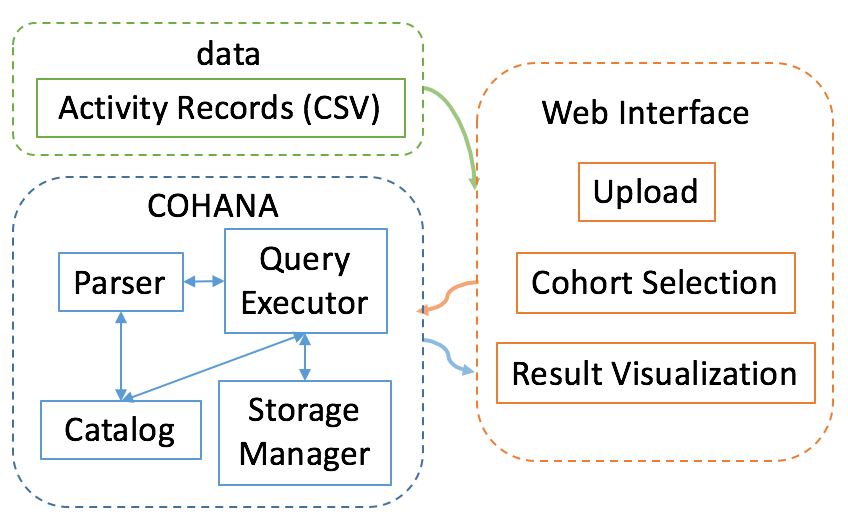
\includegraphics[width=0.4\textwidth]{arch.png}
    \caption{System Architecture}
    \label{fig:sys_arch}
\end{figure}

Figure \ref{fig:sys_arch} outlines the system architecture of the entire system. The input of the system is the data in the green rectangle and there are two components of the system, i.e., the COHANA engine and the web interface as marked as blue and orange rectangle, respectively. 

The input of the system is actually a file containing the all the user records in the CSV format. 
Besides user activities and the occurrence time, the file can also 
%The only data we required is a CSV file of user activity records, 
include the user details such as User ID, gender, etc. 
The data records are sorted by user id, and the records for each user are sorted in chronological order. 
The sorting alignment for the records is a ubiquitous format for data analysis, and it aids the COHANA engine in the detection of the tuples containing the users' birth activities.

The COHANA engine consists of a parser, a catalog, a query executor and a storage manager, wherein the last two components are the cores to support efficient cohort analysis queries. 
Compared to the original system presented in ~\cite{jiang2016cohort}, new functionalities are added to further make the query result much more readable and traceable.
For example, the user can name the cohort, or the set of cohorts, generated by the query and use the name thereafter.
This is helpful for medicians to find the effective target for a new medicine. 
A practical use case can be: the medician first locate the set of effective diseases of a medicine by COHANA and name the results by the name of diseases. Then, the medician can look into one specific diseases and further categorize the patients in the cohort of this disease by their ages, genders, diagnosing histories, etc.
% such as the birth-user selection, which is  of qualified users, the age selection operator to retrieve activity tuples satisfying certain conditions, and the cohort aggregation operator to apply certain metrics on tuples.

The storage manager applies a chunking scheme and a series of compression techniques. Specifically, they partition the data horizontally as chunks such that each chunk has approximately the same number of activity records and all activity records of a single user are included in a single chunk. Afterwards, different compression schemes are employed on each column depending on the data type of this column, e.g., Run-Length-Encoding technique is used for user identity column while two-level compression is used for string columns. For columns containing integers, delta encoding scheme is employed. 

The query executor generates a logical query plan using an operator tree from the original cohort query and optimizes the plan by pushing the birth selection into the bottom level of the tree. After being scanned on each data chunk in the storage manager, the query executor merges and presents the results of the submitted query.

The query processing in COHANA is extremely fast compared to traditional approaches in SQL due to the customized storage layout in storage manager and optimized cohort operators in query executor. As reported in~\cite{jiang2016cohort}, it is 10x and 100x faster than SQL solutions in MonetDb\cite{boncz2005monetdb} and Postgresql\cite{momjian2001postgresql}, respectively.

The interactive web interface for COHANA is implemented under Django\cite{django} framework with Gentelella\cite{gentelella} template. We also employ ECharts 2.0\cite{echarts}, a charting library, to support massive chart manipulations in our system. 
The web interface is responsible for all front-end user interactions such as uploading the dataset, constructing queries, and displaying visualized results. 
It is also in charge of back-end data transfer and interactions with COHANA engine. 

When applying the cohort analysis for their own dataset, users first specify the dataset to be analyzed via the user interface.
The back end receives the dataset and pass its address to the COHANA engine, and extracts the neeeded column information for compression in the cohort analysis page. 
Then, the users map their wanted queries from natural language to cohort definitions via the web interface, including the birth event, cohort selection, and age constructors.
The mapping is done easily with simple and clear options provided in the front end.
Next, the options selected are translated into the format acceptable by COHANA engine on the back end. Finally, the processed result is sent back from COHANA engine and parsed and visualized on the web page.

\section{Demonstration Outlines}

We will elaborate on the data preparation, the query selection, and result visualization with the aforementioned medical example in the Introduction section to explain cohort analysis process using our system since the example is quite typical for medical uses according to the doctors collaborated with us.
Although the data we use for this demonstration is not real due to the confidential issues, we indeed force the fake dataset follow the schema of the real health care records and the distribution of the original dataset (if possible).
It is worth mentioning that while the example resides in the medical domain, such analysis is common in various other domains and can likewise be elegantly handled by our system.

\subsection{Data Preparation}

Overall, we have eight columns in the CSV dataset, i.e., \emph{id, birthyear, event, disease, medicine, labtest, value, and time}. \emph{id} is a unique identifier for each patient, and \emph{birthyear} and \emph{time} are unambiguous. 
\emph{Event} contains the real affairs the user experiences.
There are three options, ``diagnose", ``prescribe" and ``labtest" in the \emph{event} column.
The \emph{disease} column contains a particular code for the illness diagnosed when a patient is admitted if the \emph{event} is ``diagnose", otherwise it is a default value set by the user.
A fact in the reality here is that even though a patient can be in the hospital for more than one day, he or she might have only one recorded diagnosis for the entire visit. 
The \emph{medicine} column indicates the prescription issued to the patient and may not cover all the days of his hospitalization. 
The \emph{labtest} refers to the type of tests patients take and the \emph{value} declares the integral test result. 

An example in the dataset is shown in Figure \ref{fig:upload}. The patient with id P-0 was admitted to the hospital on 1st January 2012, diagnosed with Disease-B, prescribed Medicine-C, and scored 44 on Labtest-C. On the next day, he scored 25 on the same lab test. 
It is worth noting that there exist redundancies in the records, which is common for real medical situations. 
The storage manager in the COHANA engine will compress the data intelligently to assure low storage consumption and high query efficiency, provided the User ID, event and time columns are sorted in the manner as described in the previous section.

% \end{figure}

\begin{figure*}
\begin{subfigure}{0.3\textwidth}
    \centering
    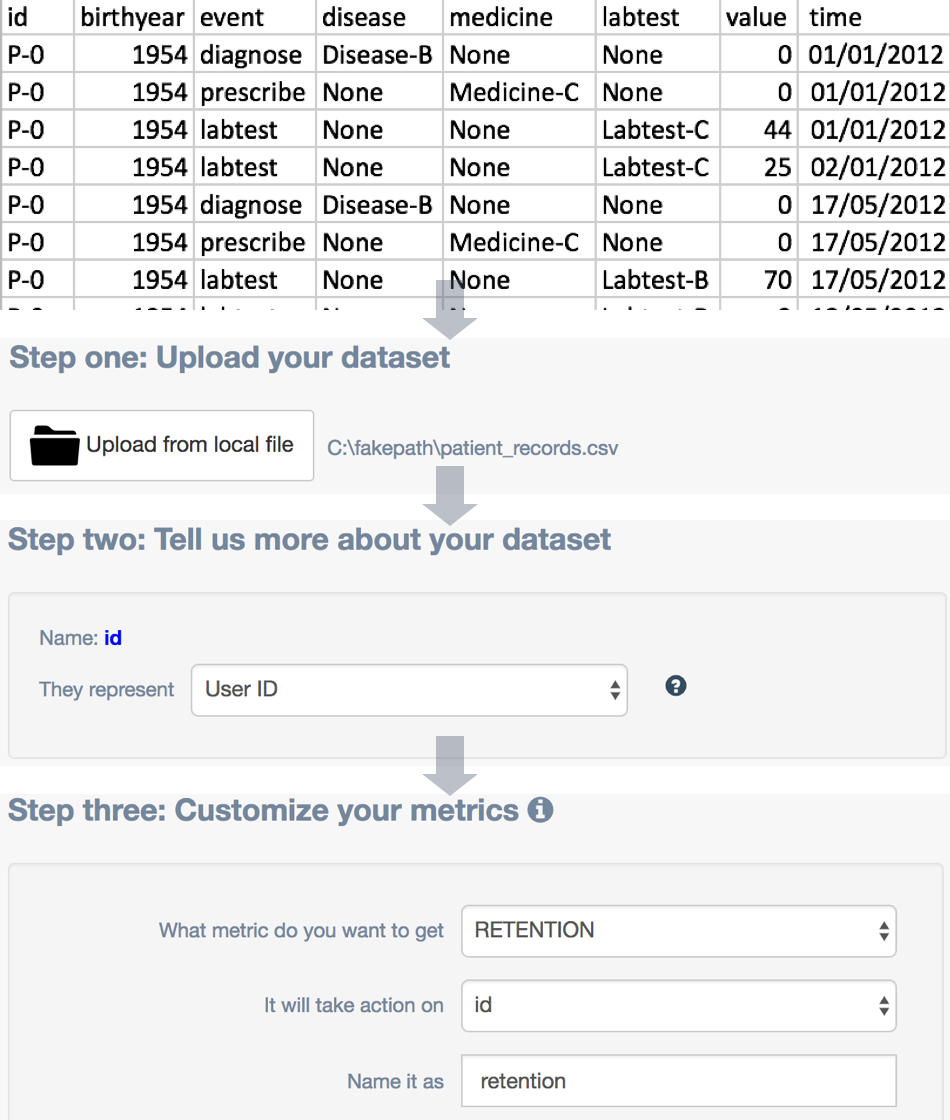
\includegraphics[width=0.9\linewidth]{upload_all_vertical.png}
    \caption{Data Upload}
    \label{fig:upload}
\end{subfigure}%
\begin{subfigure}{0.4\textwidth}
    \centering
    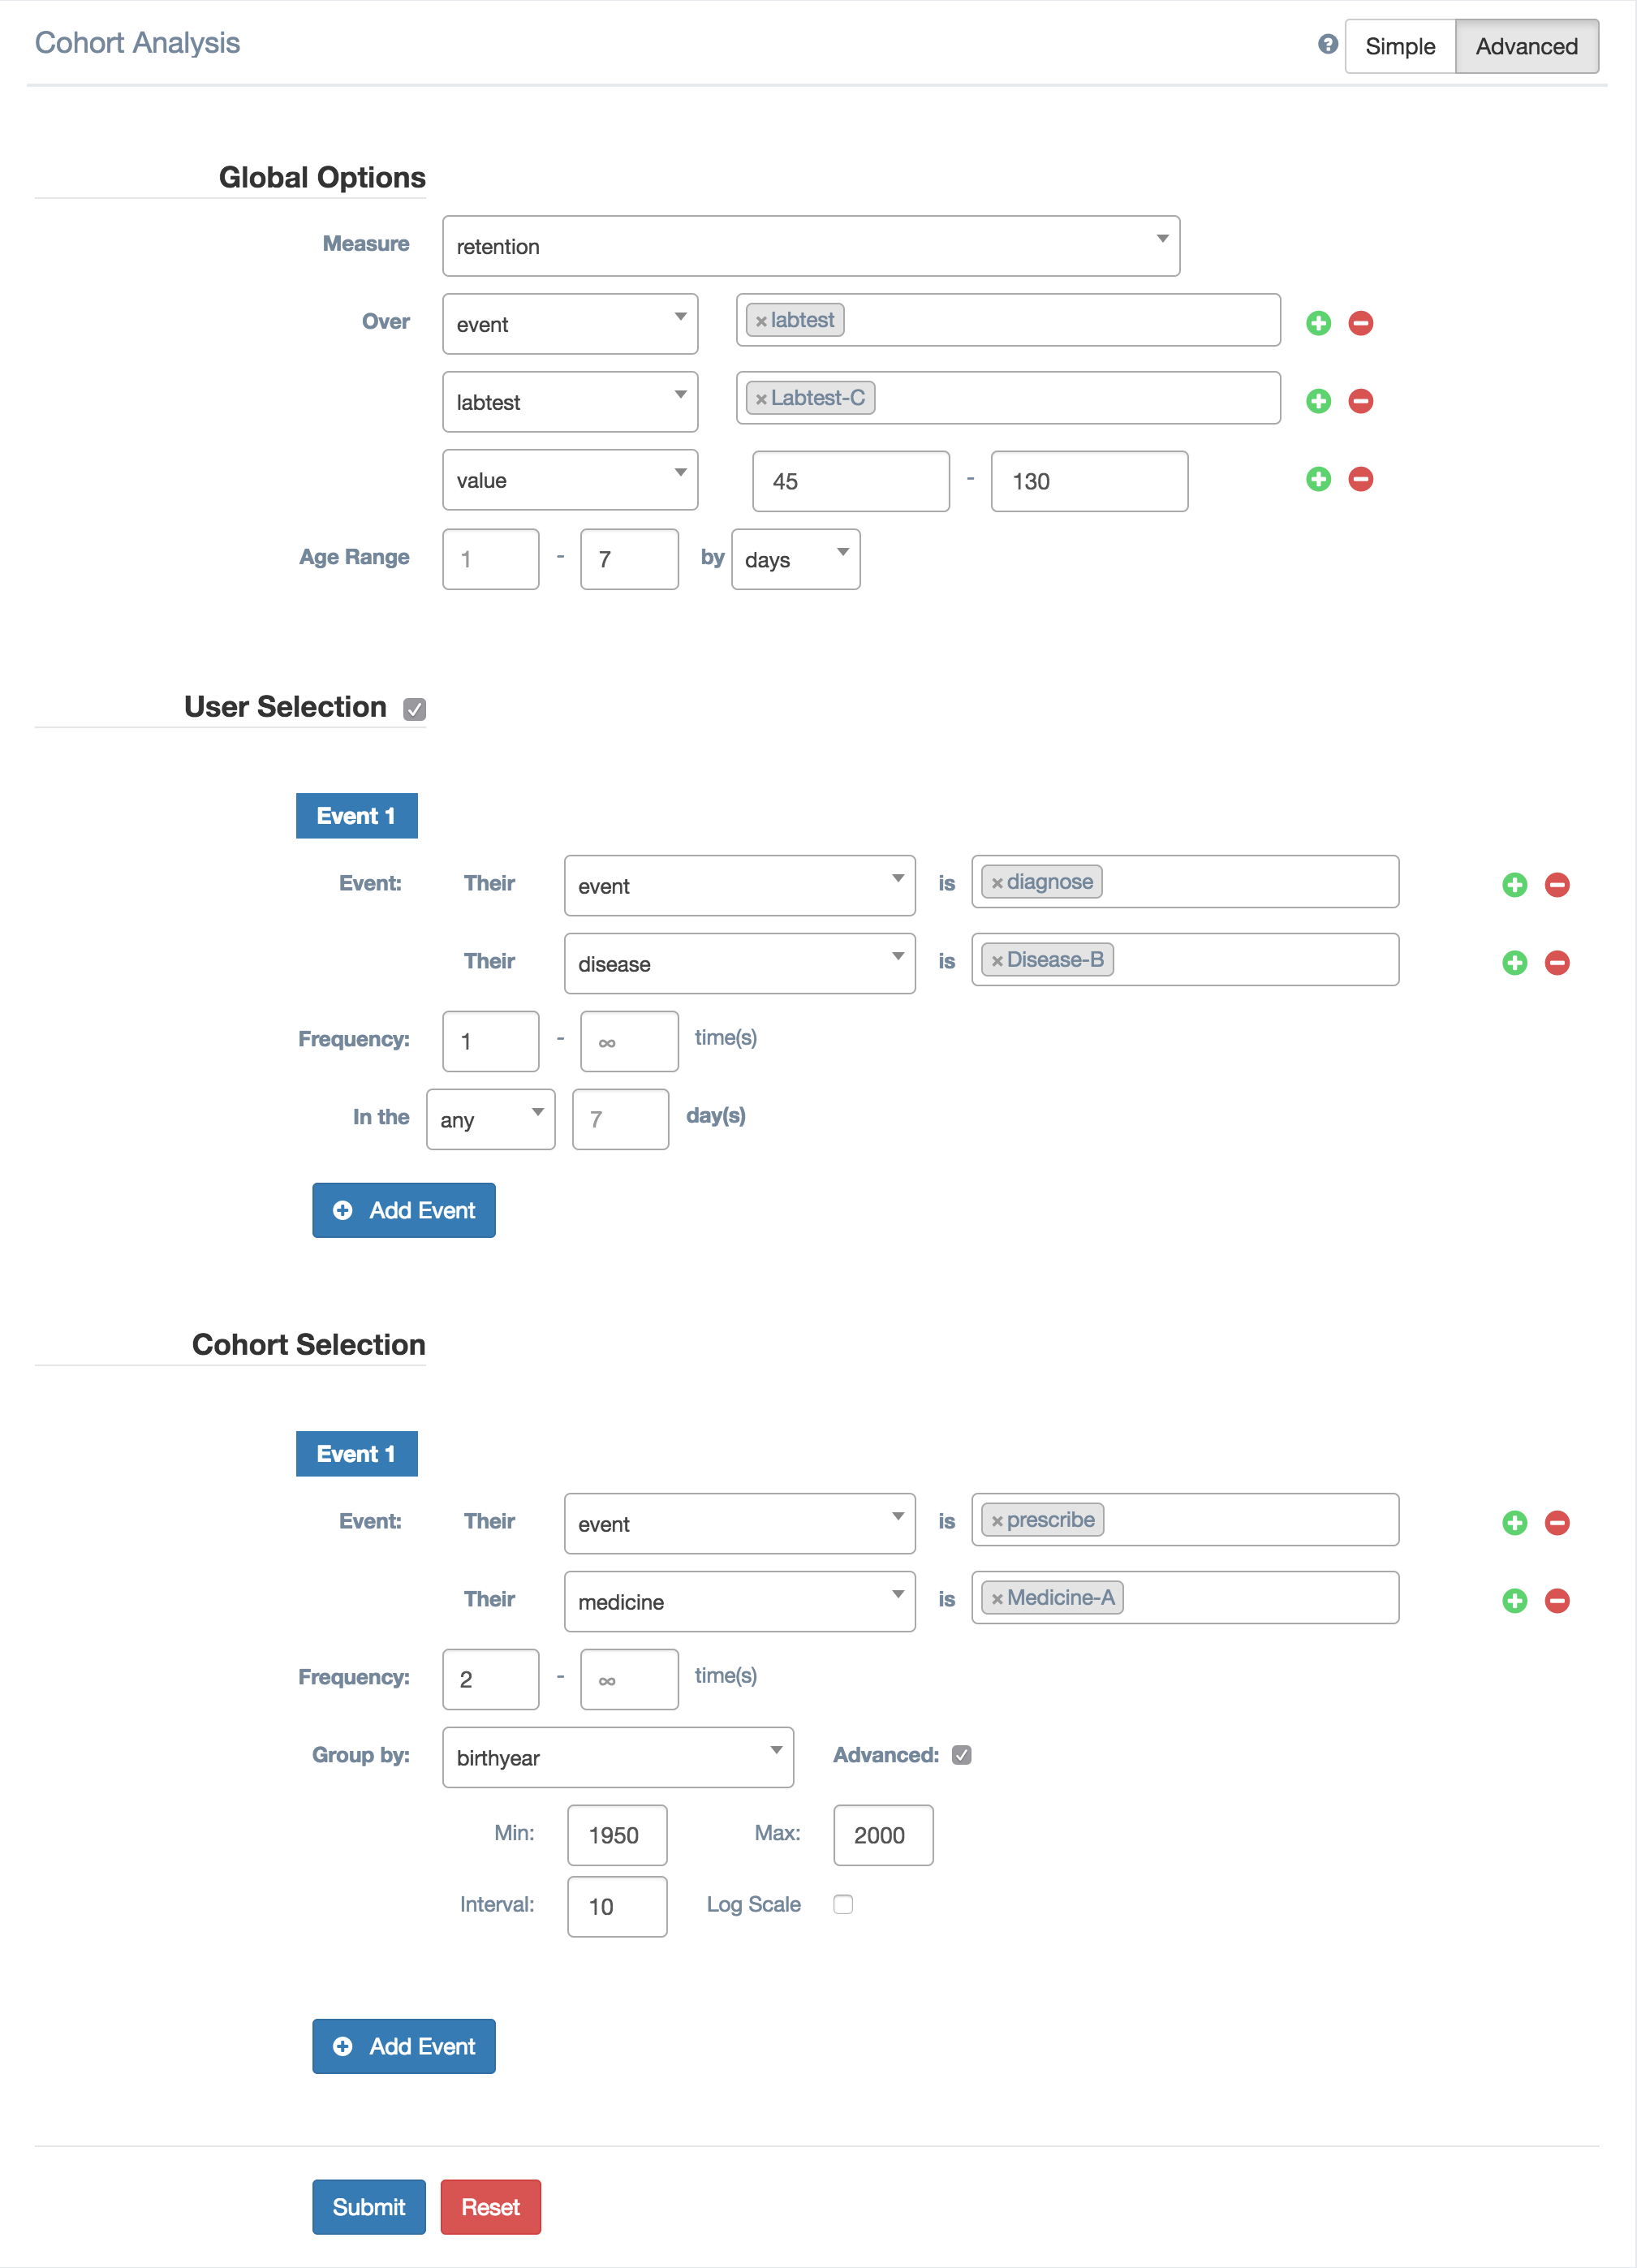
\includegraphics[width=0.9\linewidth]{query.png}
    \caption{Cohort Selection}
    \label{fig:cohort}
\end{subfigure}%
\begin{subfigure}{0.3\textwidth}
    \centering
    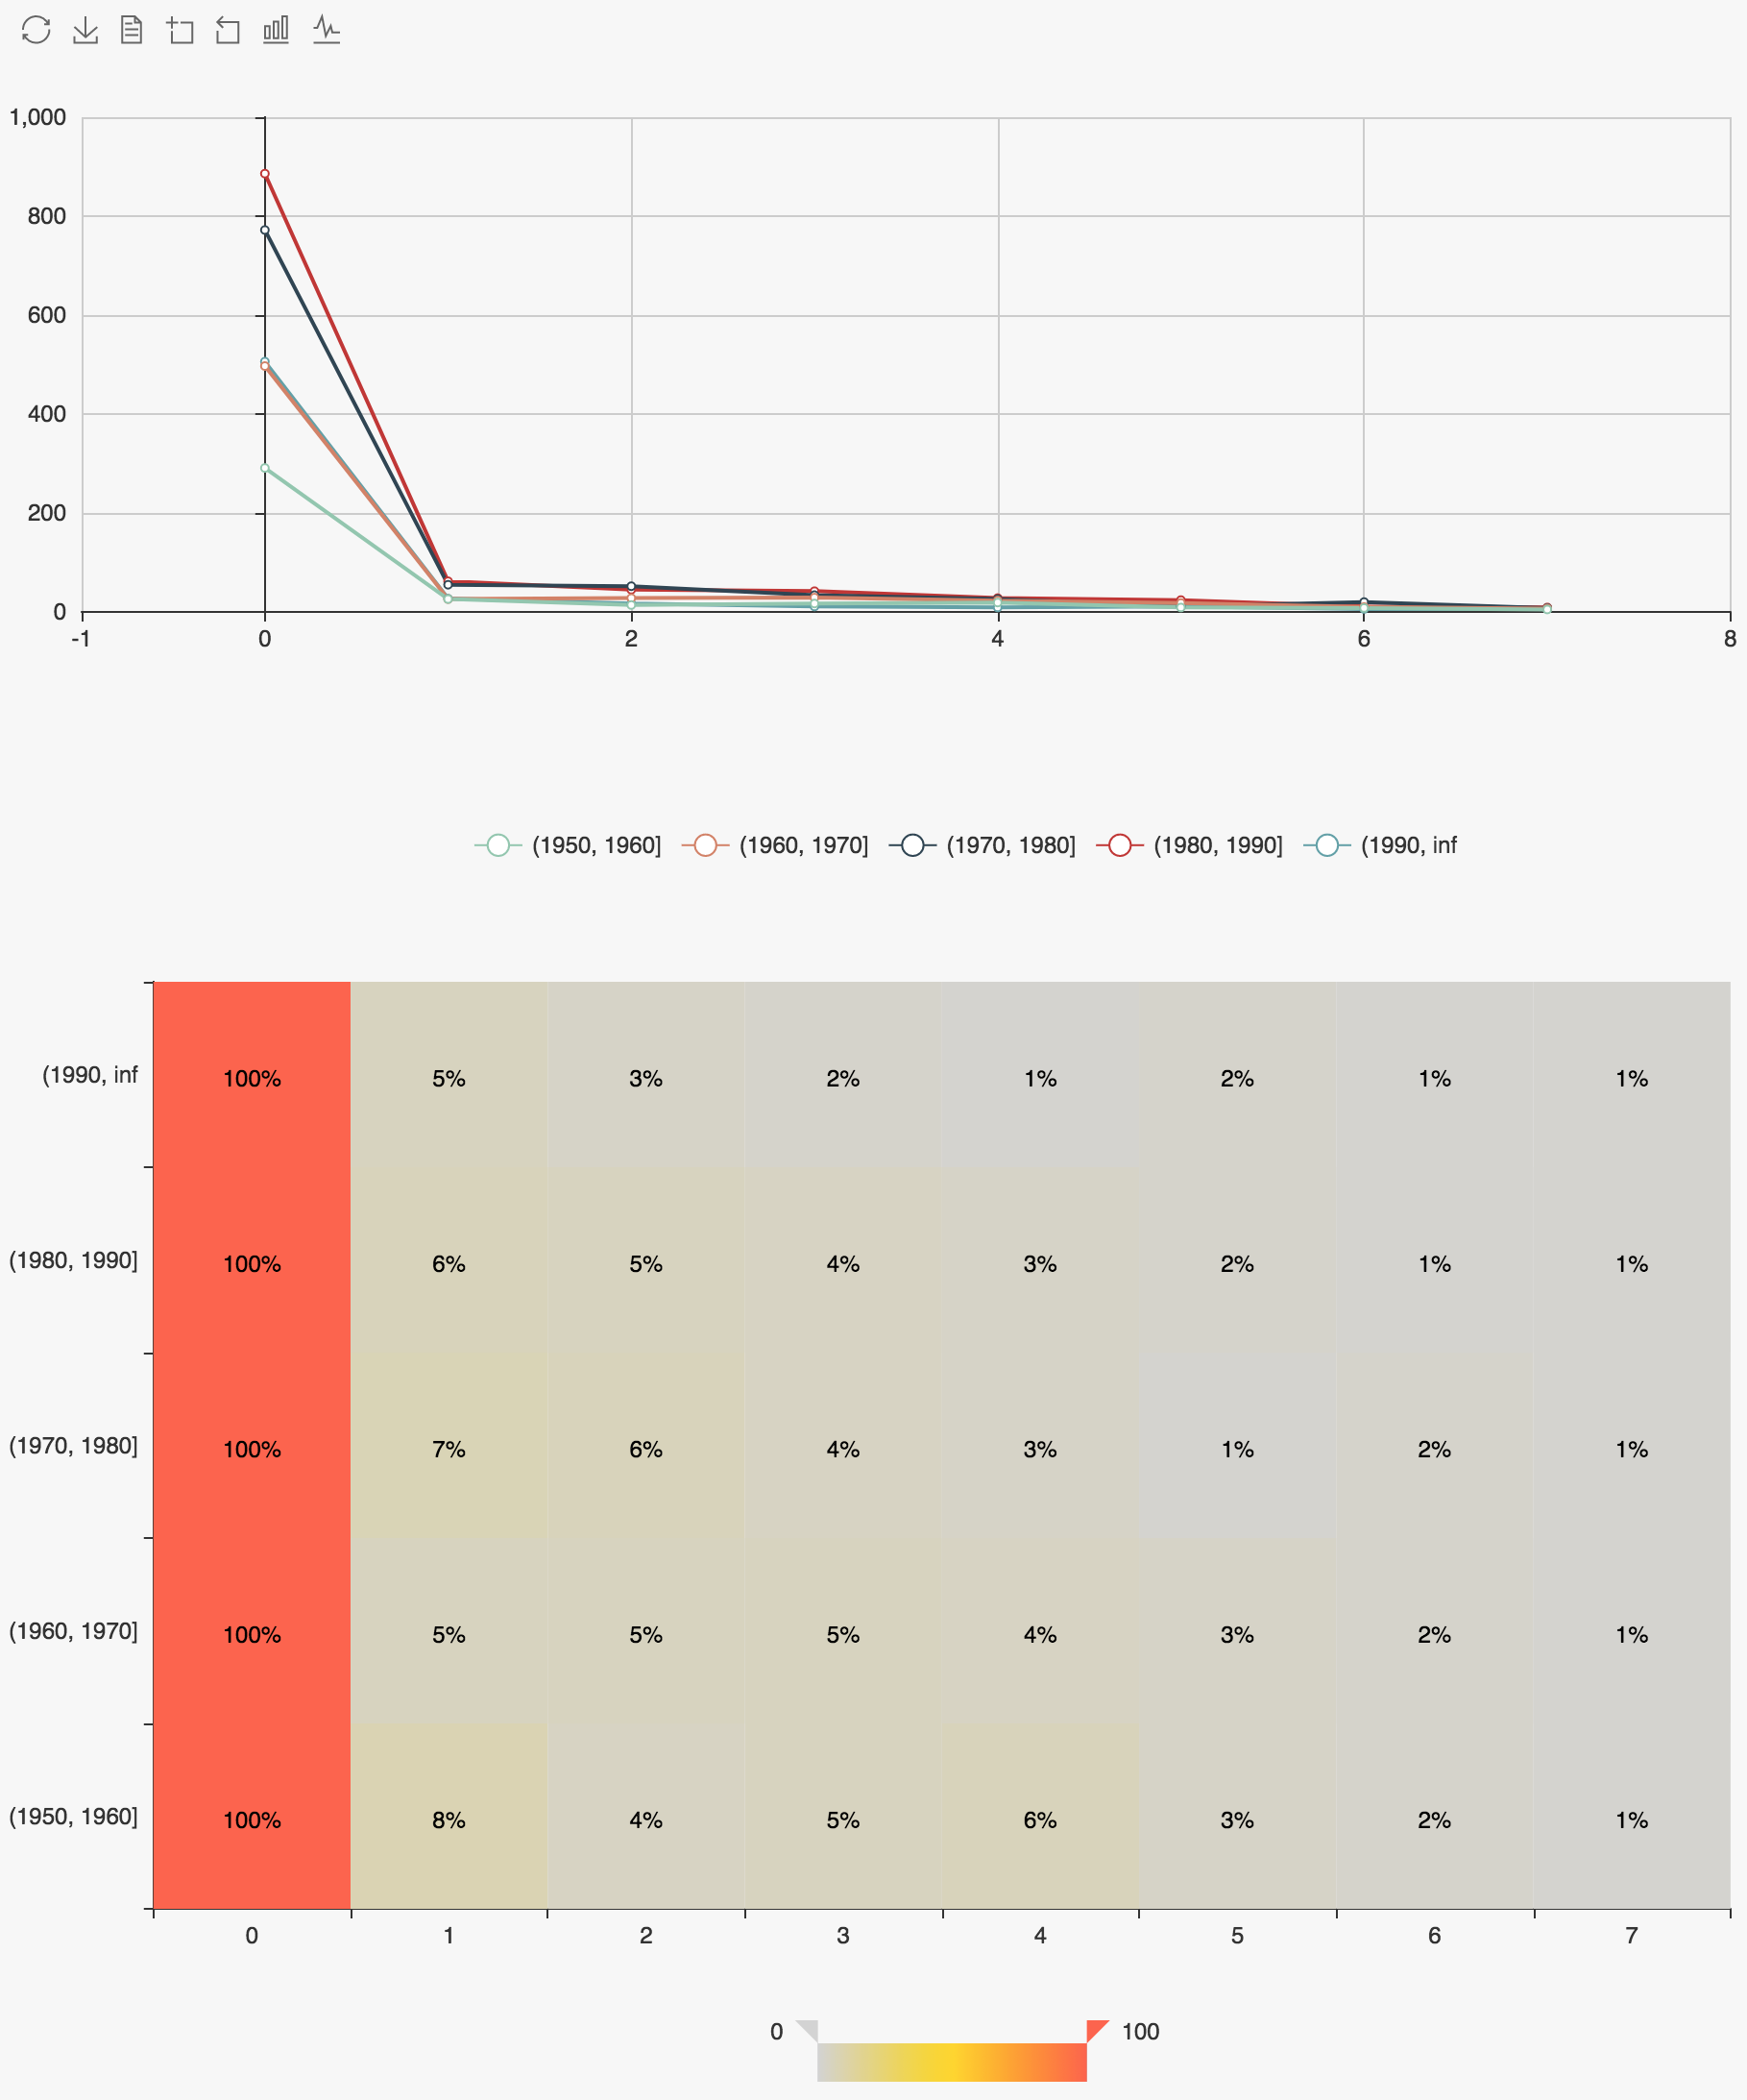
\includegraphics[width=0.9\linewidth]{chart.png}
    \caption{Result Visualization}
    \label{fig:visual}
\end{subfigure}%
\caption{Web Interface}
\end{figure*}

\begin{table}[h!]
\begin{center}
    \begin{tabular}{ |c|c| }
        \hline
        Options & Description \\[0.5ex] 
        \hline\hline
        User ID & user identity \\
        \hline
        Event & action the user performs\\
        \hline
        Event Related & other string columns\\
        \hline
        Value & other integer columns\\
        \hline
        Time & action time \\
        \hline
    \end{tabular}
\end{center}
\caption{Schema Selection for the Dataset}
\label{table:schema}
\end{table}

\begin{table}[h!]
\begin{center}
    \begin{tabular}{ | c | c | }
        \hline
        Options & Description \\[0.5ex] 
        \hline\hline
        RETENTION & number of users \\
        \hline
        COUNT & number of records \\
        \hline
        SUM & sum of certain integer column \\
        \hline
    \end{tabular}
\end{center}
\caption{Metrics Selection for the Dataset}
\label{table:metrics}
\end{table}

The first step we need to do to apply the cohort analysis is to upload the CSV file and specify the schema of the data and the metrics to be evaluated as shown in Figure \ref{fig:upload}. 
The descriptions for the options regarding the schema and metrics are shown in table \ref{table:schema} and \ref{table:metrics}. 
Here, we choose RETENTION as our metric for this problem, meaning the number of patients eligible in each cohort and age since their birth. 
The web interface allows for assigning multiple metrics, such as choosing COUNT on the labtest column if the number of abnormal values is needed, or using SUM if the total occurrences of abnormal values. 
After the COHANA engine receives the dataset and its specifications, the web application navigates the user to the cohort analysis page where options are equipped with the content found in the records.

\subsection{Cohort Selection}

According to the example, a decomposition of the natural language can be formed: 1) only patients who are diagnosed with disease B are needed for the analysis; 2) the birth event for the patients is taking medicine A two times; 3) the time unit of age is one day; and 4) the metrics are collected by counting patients that with abnormal values in lab-test C after their birth. 
Following the decomposition, the options provided on the web page can be chosen easily, which is the proceeding step discribed in this section.

As depicted in \ref{fig:cohort}, in the ``Cohort Metric" panel, we measure the \emph{retention} defined in last step over patients who experience ``labtest" event with type ``Labtest-C" and have a score between 45 to 130. 
The measured period, namely the range of the age, is from 1 to 7 days after users' birth.
The range of the age here defines the time period to investigate after each users' birth. For instance, a small range can be chosen for short-term effects while a large range can be selected for long-term effect.

The next selection is on the group of user to include in our analysis as shown in ``User Selection" panel. This part can be omitted if the analysis is conducted over all users. 
In the figure, the patients who experience event ``diagnose" with diagnosing result ``Disease-B" within any week are specified as the target users.
More constraints on user selection can be cast by ticking the \textbf{+} button on the ``Event" line.
For example, the valid range of user records can be indicated via the web interface.

For ``Birth Criteria" panel, the birth event ``prescribe" and the corresponding medicine ``Medicine-A" are specified as shown in the figure.
In addition, the birth patient should take the medicine at least twice as the frequency of this birth event is indicated to be \emph{2-$\infty$ times}.
If multiple birth events are assigned by ticking the \textbf{+} button, a patient is regarded to be born only when all the birth events are fulfilled. 
In the last part of this panel, the user indicates that the patients should be grouped further by their birthyaer in the range of \emph{1950 to 2000} with a scale value 10.

\subsection{Result Visualization}

Within seconds of submitting the cohort selection, a line chart and a heat map of the cohort analysis result will be displayed as shown in Figure~\ref{fig:visual}. In the line chart, the x-axis represents the \emph{age} of the patients since their \emph{birth} --- the number of days after taking Medicine A twice in our context --- and the y-axis represents the aggregation result, i.e., the number of patients with abnormal values detected by Labtest-C. The value of y-axis on \emph{age 0} is the total number of patients \emph{born} to the cohort. 
Each line stands for a cohort of patients as grouped by the decade they were born in. 
This line chart, answering the cohort query numerically, not only illustrates the trend of user behavior along the time axis, but also offers a view of differing behavior among various groups. 

The bottom heat map is axised with \emph{age} and cohort group. 
Each block in the heat map represents the proportion of patients fulfilling the age selection constraints in that group and \emph{age} as compared to \emph{age 0}. 
The first column, which represents \emph{age 0}, will always have the value 100\%. 
Having the blocks be shaded with different color depths in accordance to its metric value gives spontaneous expression to the relationship between \emph{age} and user behavior and may indicate deeper insights on user behavior between different cohorts. 

The two charts explain the result of the submitted cohort query in an absolute and relative manner respectively. For example, more young patients are actively displaying side effects, suggested by the high values in group (1980, 1990] in the line chart, while elder patients take longer to get accustomed to the medicine, as elderly cohorts retain color further along the age axis in the heatmap.

Additionally, with the help of ECharts\cite{echarts}, we provide a wide variety of operations to manipulate the chart, such as zooming in and changing the chart type, as shown in the toolbar above the chart. These functions afford immediate responses to visualization exploration which is helpful for further data excavation.

\section{Related Work and Conclusion}

Recently, due to the increasing volume of internet user behavioral data, cohort
analysis has been introduced to find unusual user behavior and assist to
improve user retention rate as proposed in \cite{amplitude, mixpanel, rjmetrics}. These
products directly follow the single birth event specification, restricting the diversity and the representativeness of the cohorts generated accordingly.
Moreover, they all employ simple SQL-based implementations to analyze the cohorts, which is much slower than COHANA.

The demonstration shows a powerful and comprehensive tool on top of COHANA for cohort analysis while keeping the operations as simple and intuitive as possible. Benefiting from the high efficiency of the COHANA engine, the analyst without any backgrounds can conduct reporting or verify their ideas in minimal time with a user-friendly interface. Besides, the three cohort definitions cover a broad range of practical data analysis needs in many domains concisely. Finally, the visualization of the query results provides better understanding and deeper insights towards user behavior for the users of COHANA.

%\section*{Acknowledgment}



\bibliographystyle{IEEEtran}

\bibliography{ref_list}

\end{document}
